\documentclass[a4paper,12pt]{article}
\usepackage[utf8]{inputenc}
\usepackage{graphicx}
\usepackage{geometry} % пакет для установки полей
\geometry{top=2cm} % отступ сверху
\geometry{bottom=2cm} % отступ снизу
\geometry{left=3cm} % отступ справа
\geometry{right=3cm} % отступ слева
\usepackage[russian]{babel}
\pagestyle{empty}
\begin{document}

\begin{center}
{\small\textsc{Параллель Промышленного Программирования «П» Представляет Первенство Программистов По Патрономании}}

\vskip 3pt \hrule \vskip 10pt

\end{center}
\begin{abstract}
Участникам соревнования предстоит реализовать алгоритм, который будет руководить ботом, перемещающимся по полю в поисках патронов и сражающимся с другими игроками в мире приближающегося Армагеддона. Цель каждого игрока --- как можно дольше оставаться в живых.
\end{abstract}

\section*{Правила игры}
Имеется поле $N\times N$, на котором случайным образом расположены $B$ патронов и $P$ игроков. \\ В начале игры и перед каждым ходом все игроки получают информацию о расположении патронов и других участников раунда. Игроки ходят по очереди. В процессе хода игрок может передвинуться на одну клетку вверх, вниз, влево, вправо или остаться на месте. Если в клетке, куда он передвинулся, находится патрон, то он сразу же поднимается игроком. Если в соседней по стороне с игроком клетке находится другой игрок, происходит сражение: игрок с меньшим количеством патронов умирает, а у игрока с б\'{о}льшим количеством патронов вычитаются патроны погибшего участника. В случае одинакового количества патронов, они обнуляются и начинается следующий ход (оба игрока выживают). С некоторого хода начинается Армагеддон. Во время Армагеддона после того, как все игроки сходят, у игрового поля по часовой стрелке исчезает одна клетка, начиная с левой верхней (см. пример). Игрок, находящийся на исчезнувшей клетке, считается погибшим.
\begin{center}
\begin{figure}[h]
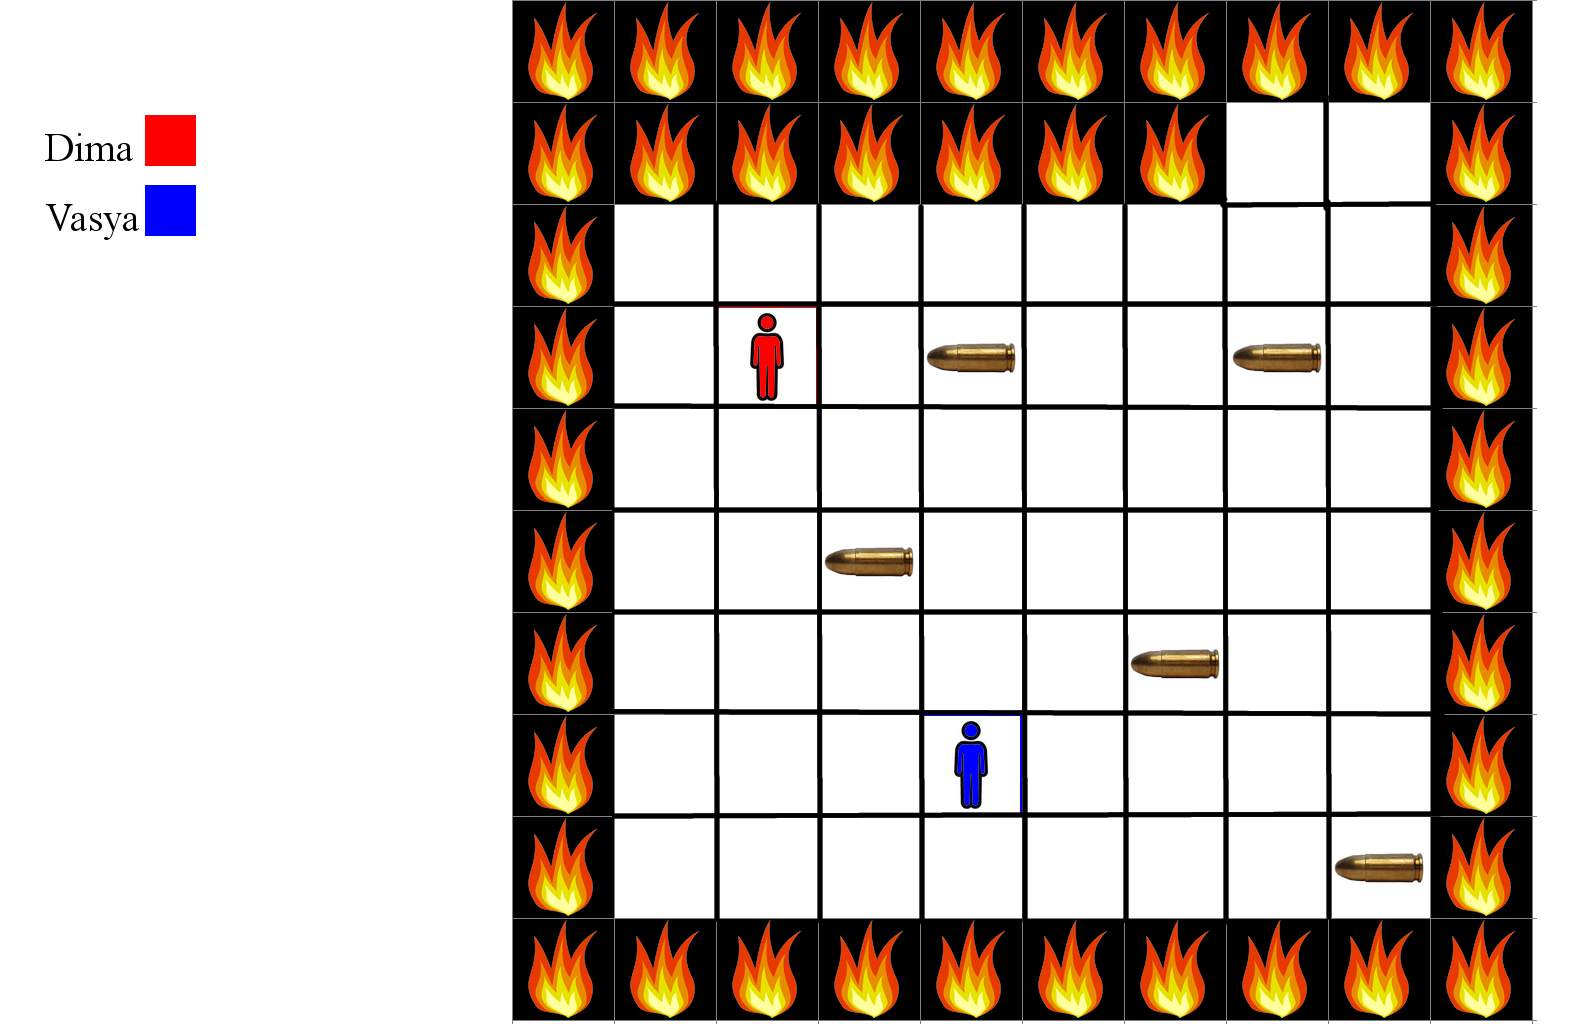
\includegraphics[width=150mm]{example1.png}
\caption{На примере Армагеддон продолжается уже 42 дня.}
\end{figure}
\end{center}

\section*{Определение победителя}
Цель игры --- продержаться на поле как можно дольше. Соответственно, победителем будет признан игрок, который на момент исчезновения игрового поля <<прожил>> больше всего ходов.
\begin{flushleft}
Игрок выбывает из игры, если его бот:
\begin{itemize}
\item погиб в результате сражения с ботом другого игрока
\item попытался выйти за пределы поля или сделал ход на поле, занимаемое другим игроком
\item не уложился в лимит времени или памяти:
TL = 1 секунда на 50 ходов, ML = 256 мегабайт
\item попытался совершить действия, которые тестирующая система сочла небезопасными
\item находился на клетке, которая исчезла
\item завершил работу до окончания игры
\end{itemize}
\end{flushleft}

\section*{Формат входного файла}
Для удобства работы будем считать, что система координат следующая:
\begin{itemize}
\item координаты верхней левой клетки: $(1;1)$
\item координаты правой верхней клетки: $(1;N)$
\item координаты правой нижней клетки: $(N;N)$.
\end{itemize}

\begin{flushleft}
В начале игры в первой строке задается размер поля $N$ ($10 \leq N \leq 50$). В процессе игры перед каждым ходом задается количество игроков $P$ ($1 \leq P \leq 2$), количество патронов $B$ ($1 \leq B \leq N^2"=P$) и время, оставшееся до Армагеддона $K$ ($"=N^2 \leq K \leq 10$, пока число положительное, клетки не исчезают --- как только число станет отрицательным, Армагеддон начнется).
Во второй строке задаются координаты участника ($x_1$, $y_1$) и количество патронов $B_1$ (изначально у всех участников патронов нет).
В следующих $P"=1$ строках построчно задаются координаты других игроков вида ($x_i$, $y_i$) и количество патронов у участника $B_i$.
В последних $B$ строках задаются координаты патронов вида ($x_k$, $y_k$). Расположение патронов генерируется в начале игры случайным образом и остается неизменным.
\end{flushleft}

\section*{Формат выходного файла}
Программа участника должна вернуть направление, в котором совершает ход: <<UP>>, если нужно передвинуться на одну клетку вверх, <<DOWN>>~--- на одну клетку вниз, <<LEFT>>~--- на одну клетку влево, <<RIGHT>>~--- на одну клетку вправо или <<STAND>>, если нужно остаться на месте.

\section*{Взаимодействие с турнирной системой}
Затем программа"=решение начинает взаимодействие с турнирной системой в соответствии со следующим протоколом:
программа выводит в стандартный поток вывода одну строку, описывающую ход бота (смотрите формат вывода в разделе \textbf{Формат выходного файла}). Вывод должен завершаться переводом строки и сбросом буфера потока
вывода. Для этого используйте:
\begin{itemize}
\item flush(output) в Pascal;
\item cout.flush() в C++;
\item import sys
      
      sys.stdout.flush() в Python 3.
\end{itemize}
После этого программа должна считать из стандартного потока ввода ответ тестирующей системы, описанный в разделе \textbf{Формат входного файла} (повторно выводится вся информация, кроме размера поля~--- он указывается только в начале игры).
\end{document}